\documentclass[11pt]{article}
%% Useful packages
\usepackage[utf8]{inputenc}
\usepackage[a4paper,left=2cm,right=2cm,top=2cm,bottom=2cm]{geometry}
\usepackage{crop,graphicx,amsmath,array,color,amssymb,fancyhdr,lineno,float,booktabs}
\usepackage{flushend,stfloats,amsthm,chngpage,times,,lipsum,lastpage,parskip,adjustbox} 
\usepackage{calc,listings,color,wrapfig,tabularx,longtable,multirow,enumitem,commath,siunitx}
\usepackage[table,xcdraw]{xcolor}
\usepackage[version = 4]{mhchem}
\usepackage[numbers]{natbib}
%\usepackage[subtle]{savetrees}
\usepackage[
  nottoc
  %notlot
  %notlof
]{tocbibind}

\usepackage{hyperref}
\hypersetup{
    colorlinks=true,
    linkcolor=black,
    filecolor=teal,      
    urlcolor=teal,
    citecolor=teal,
    pdftitle={MECH0074 Extreme Temperature Coursework},
    pdfauthor={Hasha Dar},
}

\renewcommand\bibname{References}
\usepackage{lineno}
%%%%%%%%%%%%   Header and Footer  %%%%%%%%%%%%%
\pagestyle{fancy}
\fancypagestyle{plain}{%
  \setlength{\headheight}{20pt}
}

\title{%
  }
\author{Hasha Dar\\
\textit{Student number:}\\ 
19090799
}

\begin{document}
\begin{titlepage}

  \newcommand{\HRule}{\rule{\linewidth}{0.5mm}} % Defines a new command for the horizontal lines, change thickness here

  %----------------------------------------------------------------------------------------
  %	LOGO SECTION
  %----------------------------------------------------------------------------------------
  \center
  
\includegraphics[width=5cm]{Title/UCL.png}\\[1cm] % Include a department/university logo - this will require the graphicx package

  %----------------------------------------------------------------------------------------

  \center % Center everything on the page

  %----------------------------------------------------------------------------------------
  %	HEADING SECTIONS
  %----------------------------------------------------------------------------------------

  \textsc{\LARGE University College London }\\[1.5cm] % Name of your university/college
  \textsc{\Large MEng Mechanical Engineering  }\\[0.5cm] % Major heading such as course name
  \textsc{\large MECH0071 Electrical Power Systems and Electrical Propulsion }\\[1.5cm] % Minor heading such as course title

  %----------------------------------------------------------------------------------------
  %	TITLE SECTION
  %----------------------------------------------------------------------------------------
  \makeatletter
  { \huge \textsc \@title}\\[1.5cm] % Title of your document


  %----------------------------------------------------------------------------------------
  %	AUTHOR SECTION
  %----------------------------------------------------------------------------------------

  \begin{minipage}{0.4\textwidth}
    \begin{flushleft} \large
      \emph{Author:}\\
      \@author % Your name
      \\[1.2em]
      %\emph{ID No:}\\
      %0101010 \\[1.2em]
    \end{flushleft}
  \end{minipage}
  ~
  \begin{minipage}{0.4\textwidth}
    \begin{flushright} \large
      \emph{Module coordinator:} \\
      Prof. Richard Bucknall \\[1.2em] % Supervisor's Name
      %\emph{Module teaching team:} \\
      %Dr. Tim Hillel\\ % second marker's name
      %Mr. Umut Lagap
    \end{flushright}
  \end{minipage}\\[2cm]
  \makeatother

  % If you don't want a supervisor, uncomment the two lines below and remove the section above
  %\Large \emph{Author:}\\
  %John \textsc{Smith}\\[3cm] % Your name

  %----------------------------------------------------------------------------------------
  %	DATE SECTION
  %----------------------------------------------------------------------------------------

  {\large \today}\\[2cm] % Date, change the \today to a set date if you want to be precise

  \vfill % Fill the rest of the page with whitespace

\end{titlepage}

\fancyhf{}
\fancyhead[L]{MECH0074 Extreme Temperature Coursework}
\fancyfoot[L]{Hasha Dar}
\fancyfoot[R]{ \bf\thepage\ \rm }%

\newpage
\tableofcontents
\listoffigures
\listoftables
\newpage

\section{Influence of temperature on the response of a straight pipe}
\subsection{Meaning and significance of stress terms}
\subsubsection{Principal stress}
Principal stress is a measure which defines the maximum normal stress which may be applied to a body of interest and where that stress is located. %Principal stress acts on the principal plane (an oblique plane at some angle $\theta$) and has the condition that there is zero shear stress on this plane. The resultant normal stresses acting on the principal plane, $\sigma_n$, is the principal stress. The normal stress can take a maximum or minimum value.
In the 3D case, we find that there exist three principal planes (where the shear stress is zero), which are orthogonal and each have their own maximum / minimum normal stresses. From this, we can also find locations and magnitude for the maximum shear stress.

Consider the six components of the 3D solid stress tensor:
\begin{equation}
    \sigma_{ij} = \begin{bmatrix}
        \sigma_x & \tau_{yx} & \tau_{zx}\\
        \tau_{xy} & \sigma_y & \tau_{zy}\\
        \tau_{xz} & \tau_{yz} & \sigma_z
    \end{bmatrix}
\end{equation}
where the first subscript denotes the direction of the surface normal and the second the direction of the stress. For static equilibrium:
\begin{equation}
    \tau_{xy} = \tau_{yx} \qquad \tau_{xz} = \tau_{zx} \qquad \tau_{zy} = \tau_{yz}
\end{equation}
By rotating the coordinate axes of our 3D body, we can change the components of the solid stress tensor, whilst representing the same state of stress on the body. As our matrix is symmetric, we can calculate a set of orthogonal axes which result in all $\tau$ elements equalling zero. This set of axes is called the principal axes and by applying this transformation to our solid stress tensor, we find the eigenvalues of the matrix and the principal stresses. Hence:
\begin{gather}
    \boldsymbol{\sigma}_{ij} = \begin{bmatrix}
        \sigma_x & \tau_{yx} & \tau_{zx}\\
        \tau_{xy} & \sigma_y & \tau_{zy}\\
        \tau_{xz} & \tau_{yz} & \sigma_z
    \end{bmatrix} \xrightarrow{eigenvalues} \boldsymbol{\sigma}_{ij}' = \begin{bmatrix}
        \sigma_1 & 0 & 0\\
        0 & \sigma_2 & 0\\
        0 & 0 & \sigma_3
    \end{bmatrix}\\
    \det(\boldsymbol{\sigma} - \sigma \boldsymbol{I}) = 0
\end{gather}
where $\boldsymbol{I}$ is the identity matrix and $\sigma$ is the eigenvalue. The eigenvectors of the stress tensor, which correspond to the principal directions (the angles between the original (or base) coordinate axes and the new (or transformed) coordinate axes), can be found by solving the equation:
\begin{equation}
    (\boldsymbol{\sigma} - \sigma \boldsymbol{I})\boldsymbol{v} = \boldsymbol{0}
\end{equation}
where $\boldsymbol{v}$ is the eigenvector. This may also be written as:
\begin{align}
    \cos \alpha = \cos\left(n, \, x\right) & = l\\
    \cos \beta = \cos\left(n, \, y\right) & = m\\
    \cos \gamma = \cos\left(n, \, z\right) & = n
\end{align}
where $n$ is the unit normal to the plane. We can now define the normal stress acting on any oblique plane:
\begin{equation}
    \sigma_{x'} = \sigma_xl^2 + \sigma_y m^2 +\sigma_zn^2 + 2\left(\tau_{xy}lm + \tau_{xy}mn + \tau_{xz}ln\right)
\end{equation}
We are interested in the maximum and / or minimum values of the normal stress acting on our body throughout the range of oblique planes. These maxima / minima are the principal stresses. This is determined by calculating the differentials of the above equations with respect to the direction cosines. We find that the principal stresses occur on planes where the shear stress is zero, as mentioned previously. The equations for in-plane principal stresses are shown below. The third stress is zero in plane stress conditions.
\begin{gather}
    \sigma_1 = \left(\frac{\sigma_x + \sigma_y}{2}\right)+ \sqrt{\left(\frac{\sigma_x - \sigma_y}{2} \right)^2+ \tau^2_{xy} }\\
    \sigma_2 = \left(\frac{\sigma_x + \sigma_y}{2}\right)- \sqrt{\left(\frac{\sigma_x - \sigma_y}{2} \right)^2+ \tau^2_{xy} }
\end{gather}

A key characterisation of the principal stress is that it acts in the normal direction to the principal plane - this is important to note as a distinction. The determination of the principal stresses (and maximum shear stress) is important for design purposes as it tells us whether a body would be able to withstand a design load at a given location.
\subsubsection{Von Mises stress}
\url{https://www.continuummechanics.org/vonmisesstress.html}

Von Mises stress can be used to determine whether an isotropic and ductile material will yield under a complex loading condition. It takes into account all three principal stresses (tensile, compressive, and shear) that act on a material at a particular point and provides a measure of the overall stress state at that point. A comparison between the material's yield stress and the von Mises stress allows the calculation of the von Mises Stress Criterion.

The von Mises stress is calculated by finding the square root of the sum of the squares of the differences between the principal stresses and the mean stress. Mathematically, the von Mises stress is given by:
\begin{equation}
    \sigma_{VM} = \sqrt{\frac{3}{2}\sum_{i=1}^{3}(\sigma_i-\sigma_{avg})^2}
\end{equation}
where $\sigma_i$ is the $i$-th principal stress, and $\sigma_{avg}$ is the average of the three principal stresses, given by:
\begin{equation}
    \sigma_{avg} = \frac{1}{3}\sum_{i=1}^{3}\sigma_i
\end{equation}
The mean stress $\sigma_{avg}$ is simply the average of the three principal stresses, given by:
\begin{equation}
    \sigma_{avg} = \frac{1}{3}(\sigma_1 + \sigma_2 + \sigma_3)
\end{equation}
Substituting these equations into tqhe von Mises stress equation gives:
\begin{equation}
    \sigma_{VM} = \sqrt{\frac{3}{2}\left[(\sigma_1-\sigma_{avg})^2 + (\sigma_2-\sigma_{avg})^2 + (\sigma_3-\sigma_{avg})^2\right]}
\end{equation}
This equation shows that the von Mises stress depends only on the six independent components of the stress tensor, which are the normal stresses $\sigma_{ii}$, $\sigma_{jj}$, and $\sigma_{33}$, and the shear stresses $\sigma_{12}$, $\sigma_{23}$, and $\sigma_{31}$. It is independent of the coordinate system and is therefore a useful measure of the overall stress state of a material.

The von Mises stress is often used in engineering design to determine whether a material will fail under a given load. If the von Mises stress exceeds the yield strength of the material, plastic deformation is expected to occur. Therefore, designers can use the von Mises stress to ensure that their designs remain within the elastic limit of the material.

In summary, the von Mises stress is a measure of the overall stress state of a material, taking into account all three principal stresses. It is calculated by finding the square root of the sum of the squares of the differences between the principal stresses and the mean stress. In the 3D case, the von Mises stress depends only on the six independent components of the stress tensor, and is a useful measure of the likelihood of plastic deformation in a material.
\subsubsection{Stress magnitude}
\subsection{Relationship between axial stress and temperature of length constrained 3D pipe}\label{part1b}
\subsection{3D pipe ANSYS}\label{part1c}
\subsubsection{Relationship between maximum stress in temperature range}
\subsubsection{Comparison against theoretical result and discussion}
\subsection{1D pipe ANSYS}\label{part1d}
\subsubsection{Relationship between maximum stress in temperature range}
\subsubsection{Comparison against theoretical result and discussion}
\subsection{Discussion}
\subsubsection{Difference and similarities between results from \ref{part1b}, \ref{part1c}, \ref{part1d} as pipe slenderness changes}
\subsubsection{Model errors encountered using ANSYS Static Structural model}

\newpage
\bibliographystyle{unsrtnat}
\bibliography{Refs.bib}
\appendix
\chapter{Plots}
\begin{figure}[H]
    \centering
    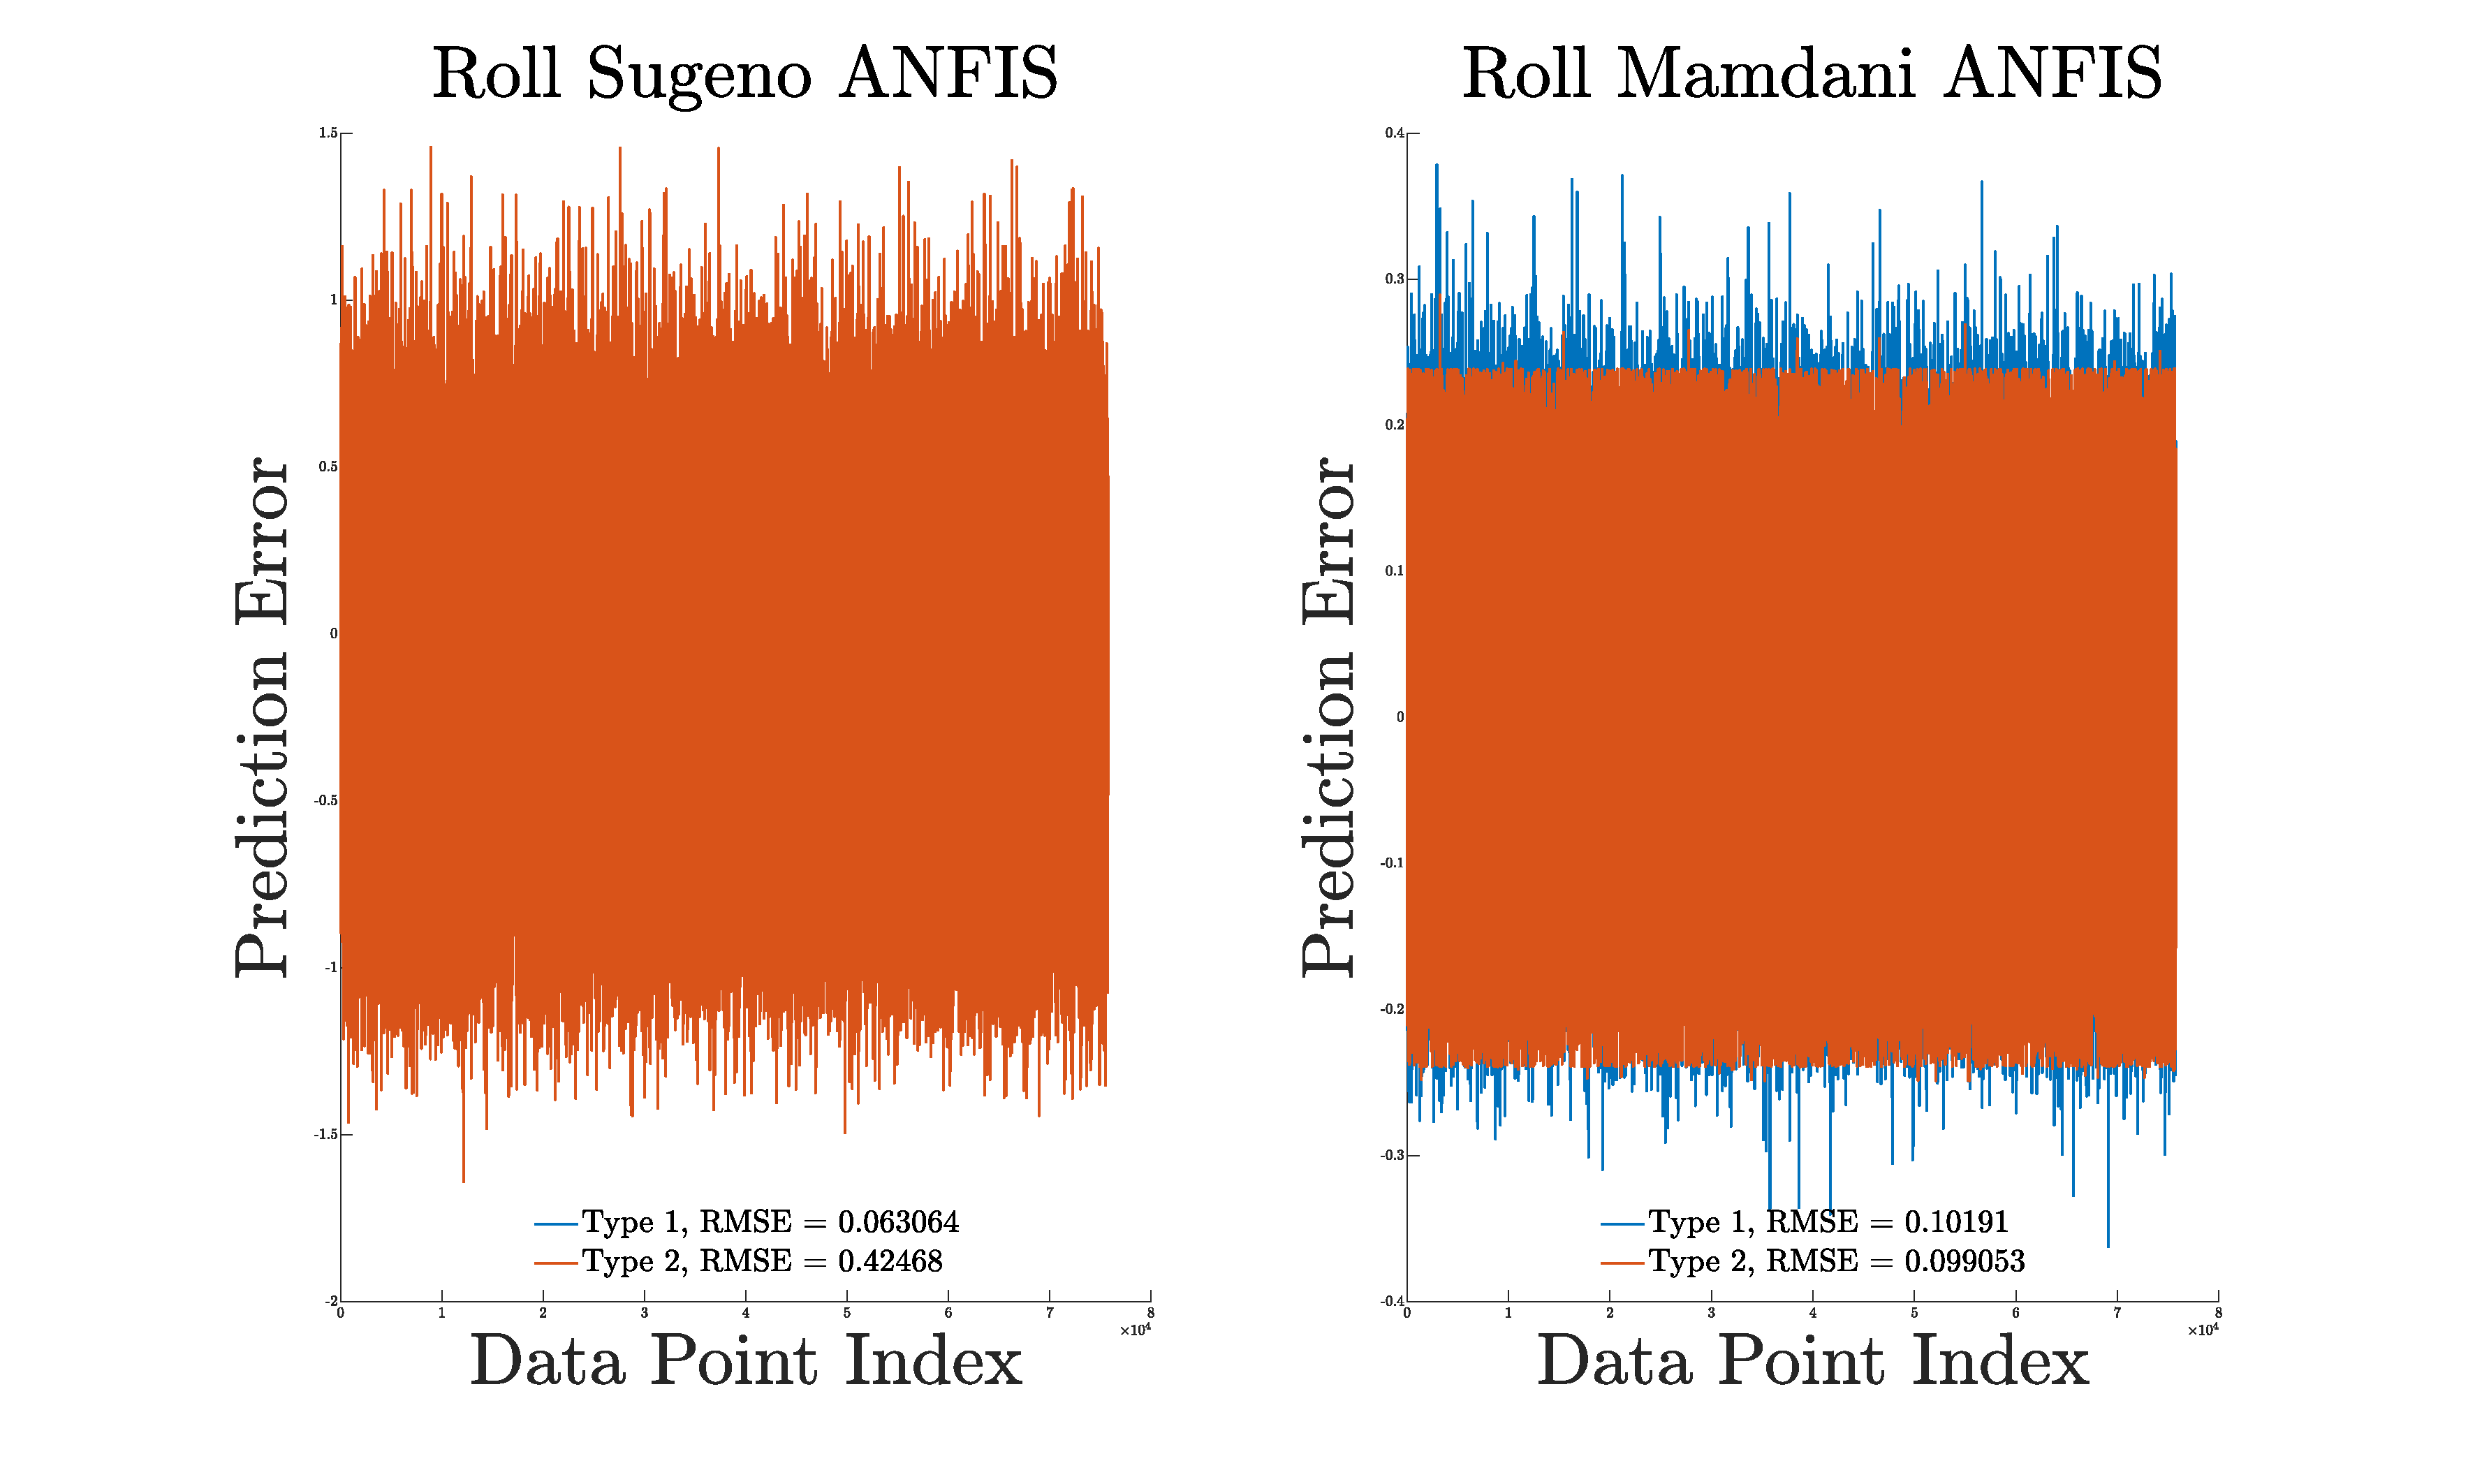
\includegraphics[width = 0.8\textwidth]{img/Roll Type.pdf}
    \caption{RMSE results for Type-1 and Type-2 Configurations for Roll Output}
    \label{fig:roll_type}
\end{figure}
\begin{figure}[H]
    \centering
    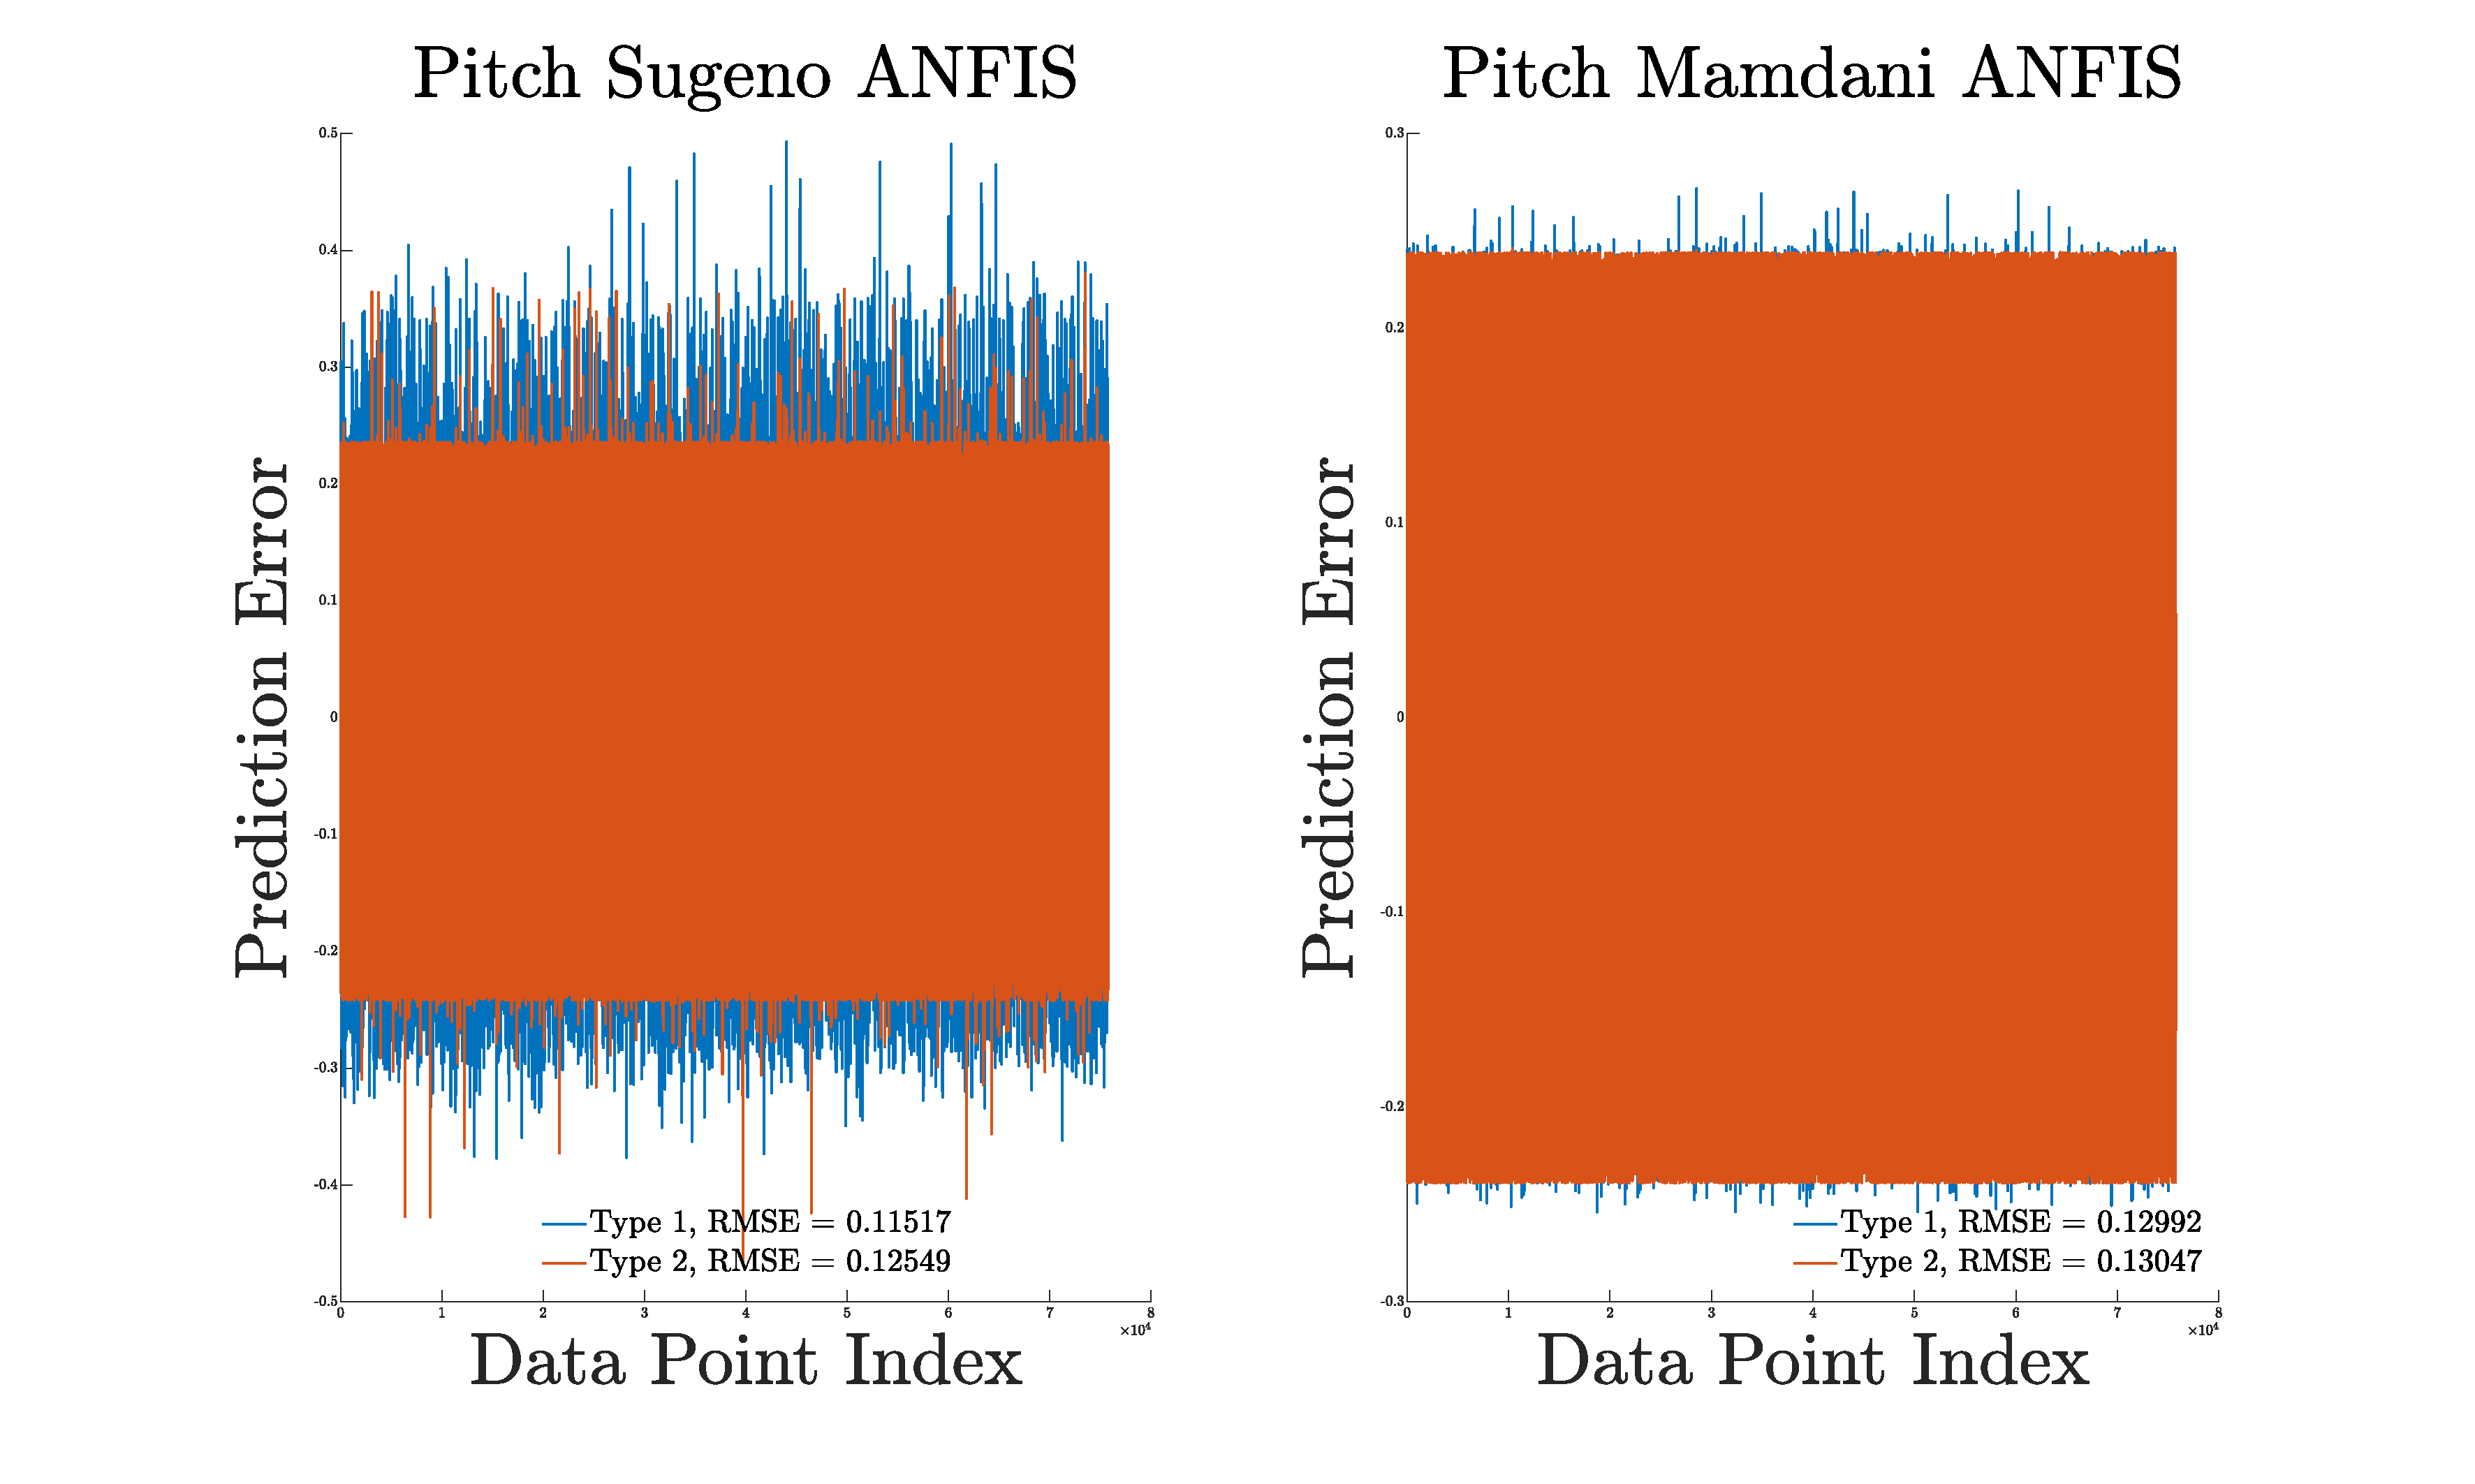
\includegraphics[width = 0.8\textwidth]{img/Pitch Type.pdf}
    \caption{RMSE results for Type-1 and Type-2 Configurations for Pitch Output}
    \label{fig:pitch_type}
\end{figure}
\begin{figure}[H]
    \centering
    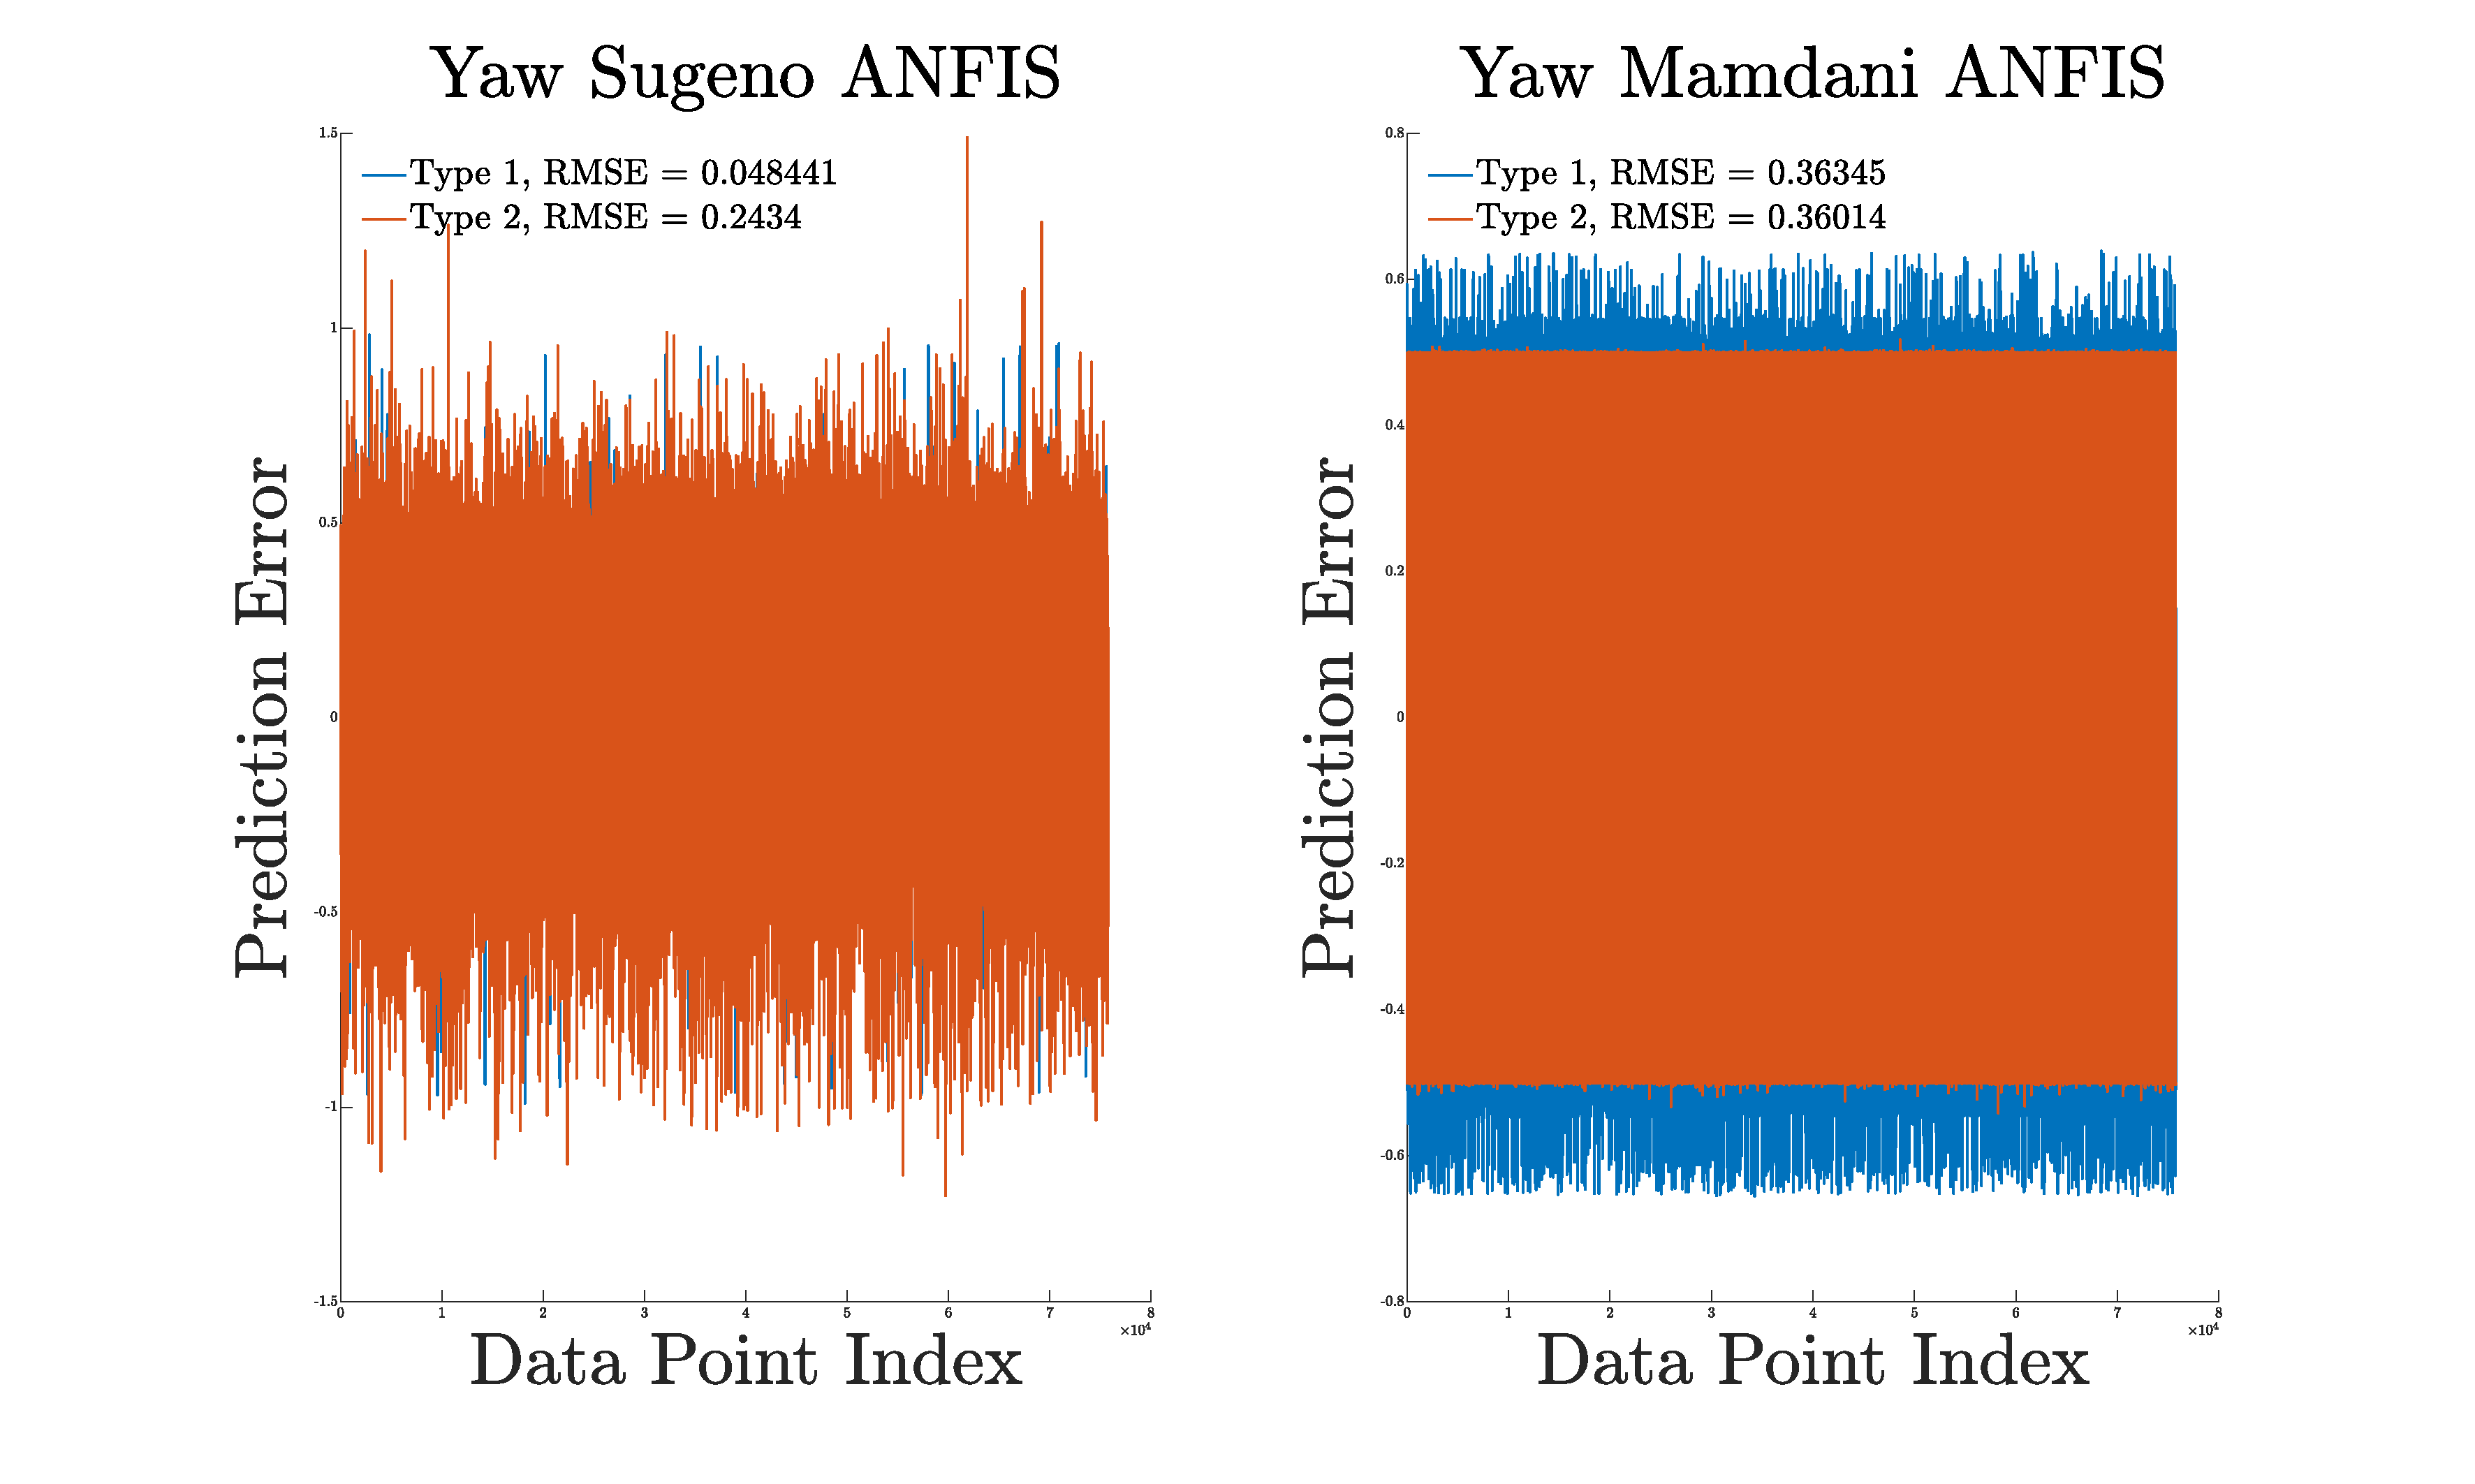
\includegraphics[width = 0.6\textwidth]{img/Yaw Type2.pdf}
    \caption{RMSE results for Type-1 and Type-2 Configurations for Yaw Output}
    \label{fig:yaw_type}
\end{figure}
\begin{figure}[H]
    \centering
    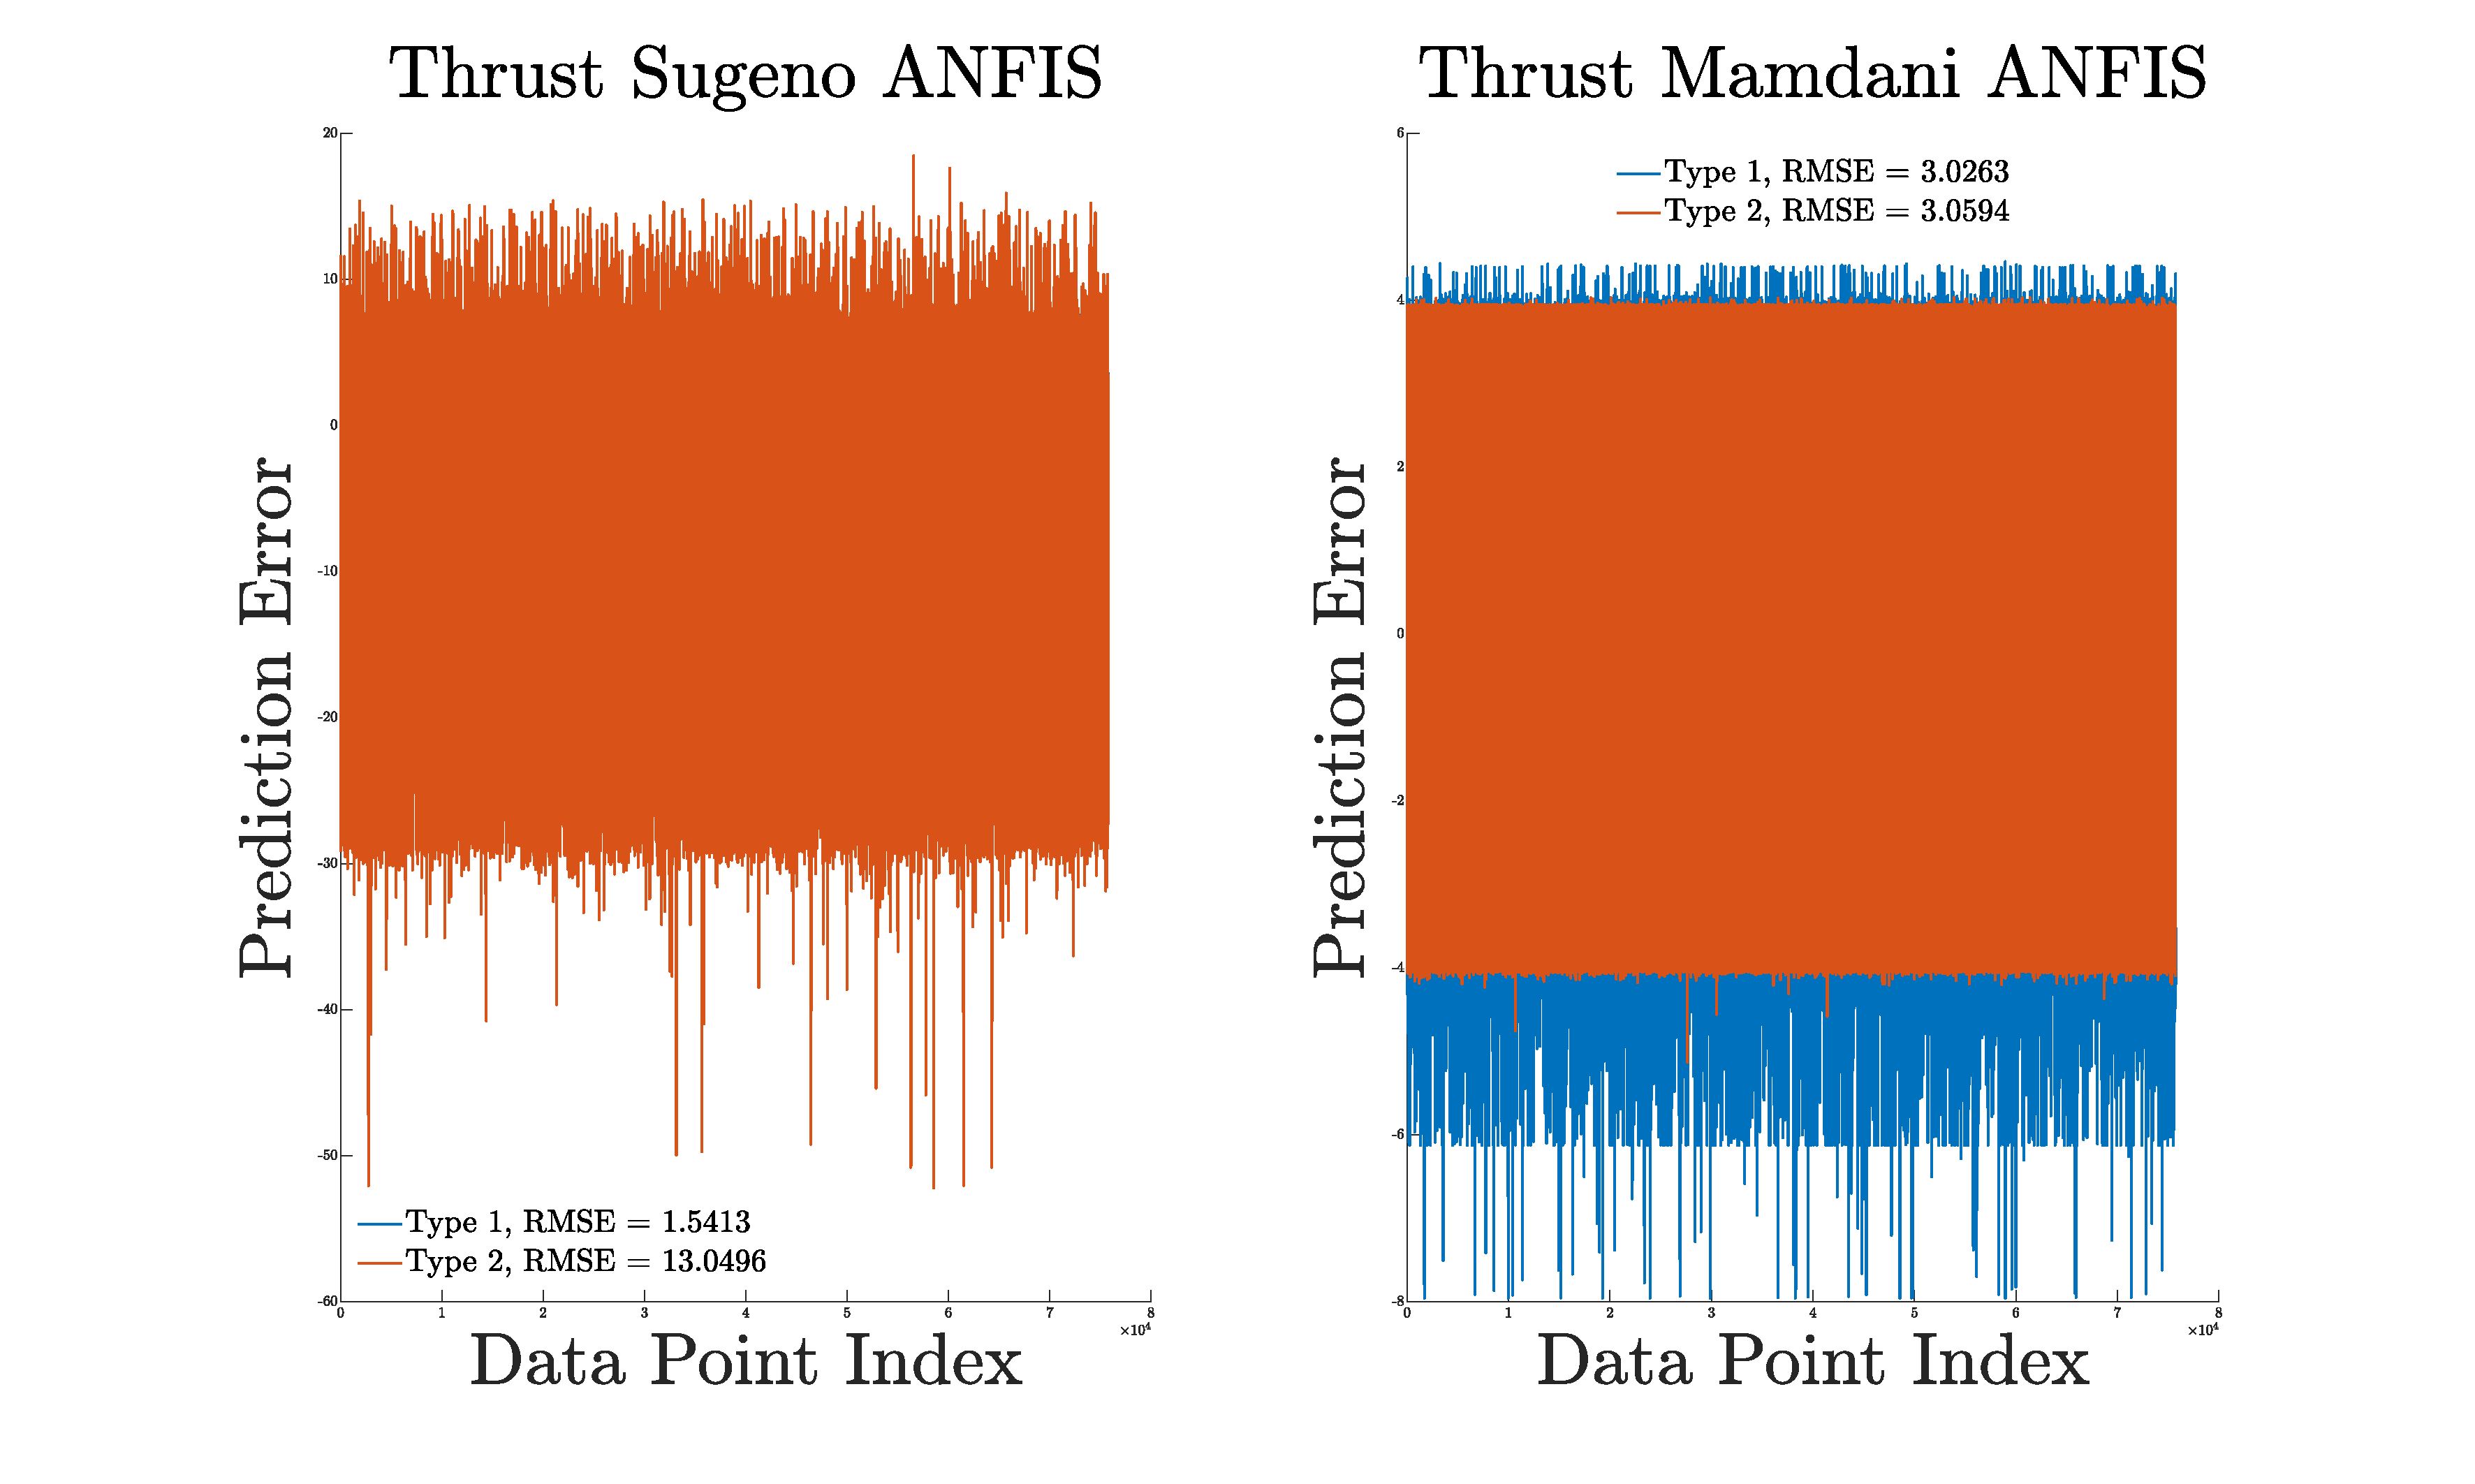
\includegraphics[width = 0.6\textwidth]{img/Thrust Type.pdf}
    \caption{RMSE results for Type-1 and Type-2 Configurations for Thrust Output}
    \label{fig:thrust_type}
\end{figure}
\begin{figure}[H]
    \centering
    \begin{minipage}[b]{0.45\textwidth}
        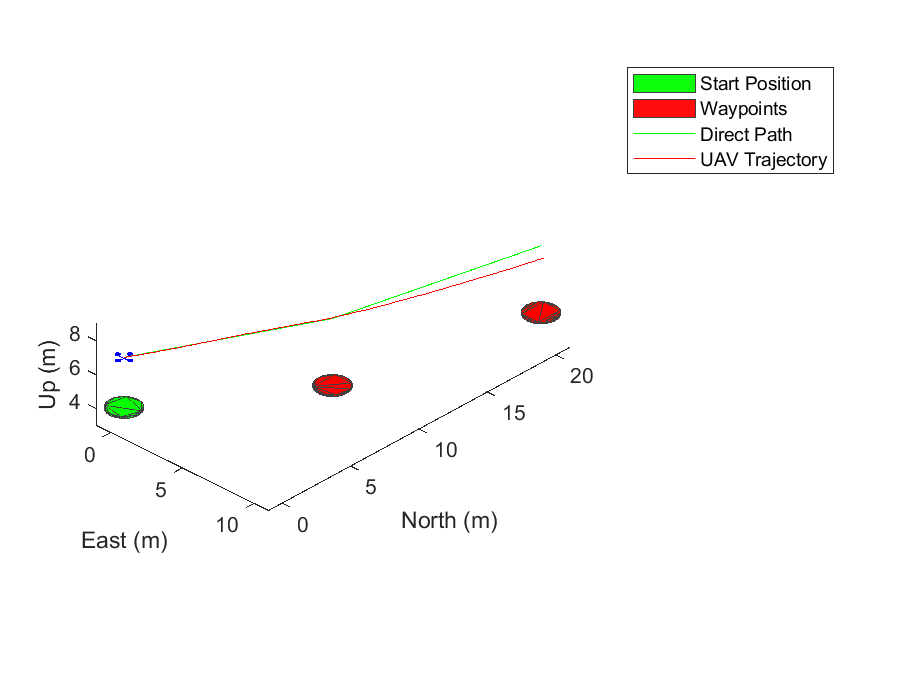
\includegraphics[height=5cm,keepaspectratio]{img/scenario1_pid_paths.eps}
        \caption{Scenario 1 Path taken using PID Drone Control}
        \label{fig:Paths1_pid}
    \end{minipage}
    \hfill
    \begin{minipage}[b]{0.45\textwidth}
        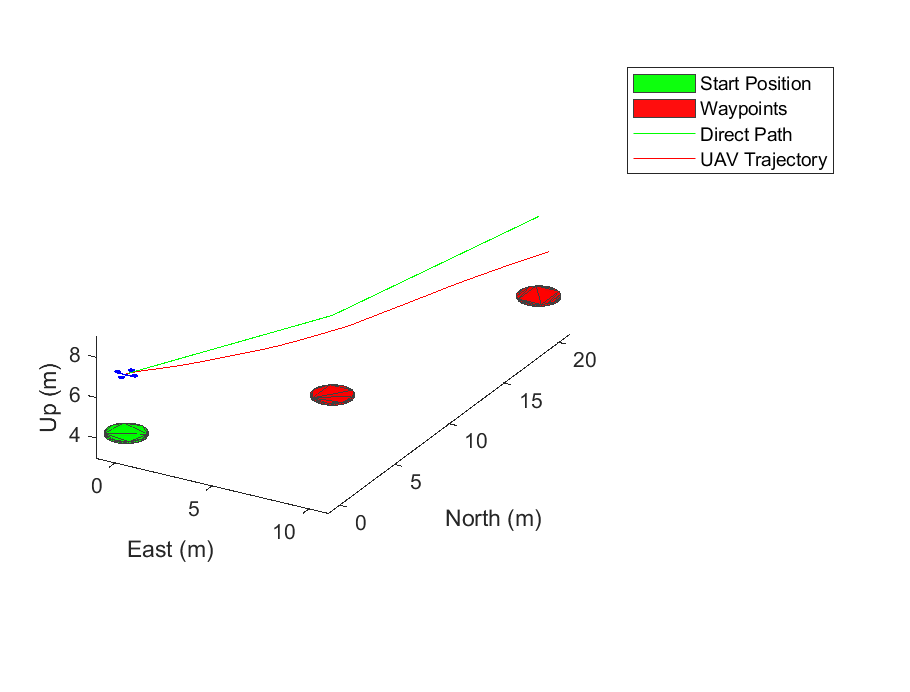
\includegraphics[height=5cm,keepaspectratio]{img/scenario1_fis_paths.eps}
        \caption{Scenario 1 Path taken using ANFIS Drone Control}
        \label{fig:Paths1_fis}
    \end{minipage}
\end{figure}
\begin{figure}[H]
    \centering
    \begin{minipage}[b]{0.45\textwidth}
        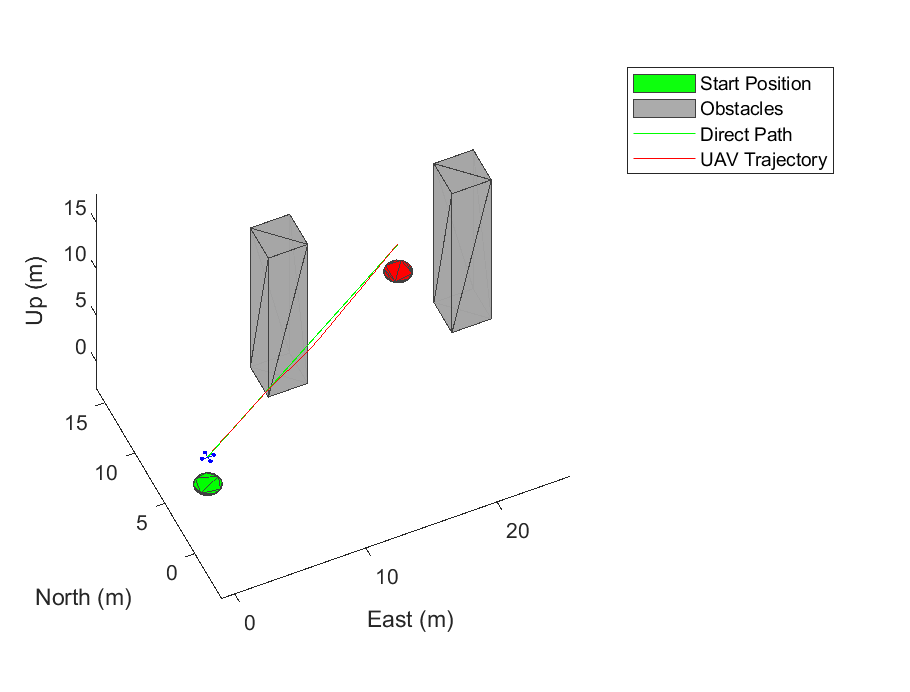
\includegraphics[height=5cm,keepaspectratio]{img/scenario2_pid_paths.eps}
        \caption{Scenario 2 Path taken using PID Drone Control}
        \label{fig:Paths2_pid}
    \end{minipage}
    \hfill
    \begin{minipage}[b]{0.45\textwidth}
        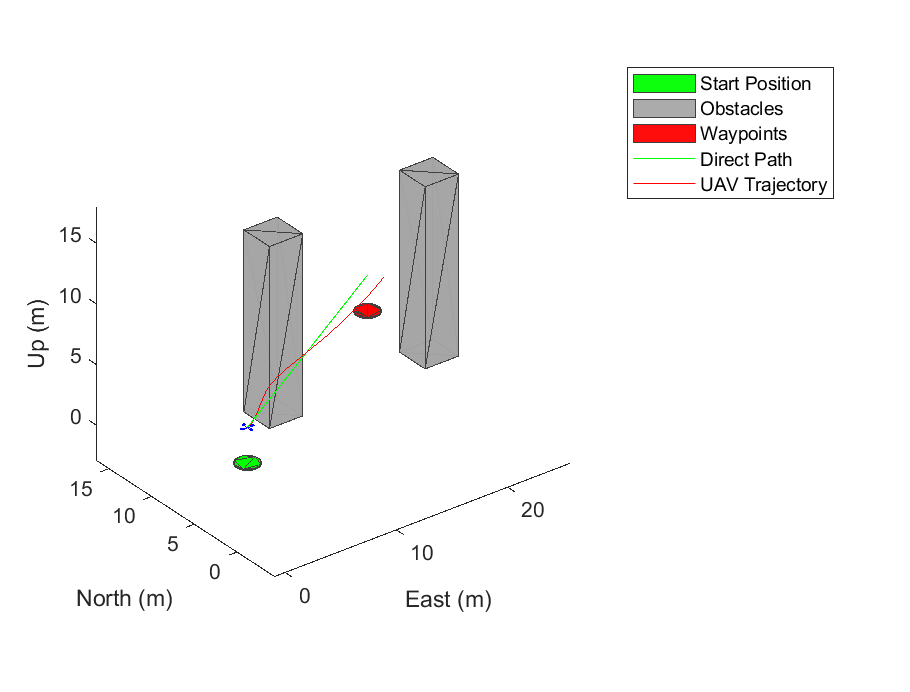
\includegraphics[height=5cm,keepaspectratio]{img/scenario2_fis_paths.eps}
        \caption{Scenario 2 Path taken using ANFIS Drone Control}
        \label{fig:Paths2_fis}
    \end{minipage}
\end{figure}
\begin{figure}[H]
    \centering
    \begin{minipage}[b]{0.45\textwidth}
        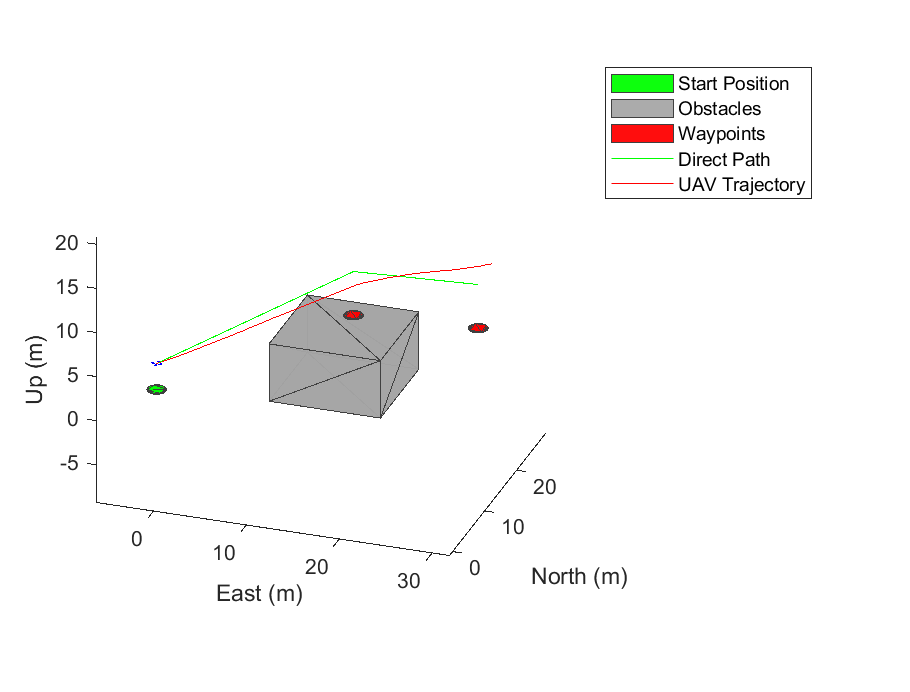
\includegraphics[height=5cm,keepaspectratio]{img/scenario3_pid_paths.eps}
        \caption{Scenario 3 Path taken using PID Drone Control}
        \label{fig:Paths3_pid}
    \end{minipage}
    \hfill
    \begin{minipage}[b]{0.45\textwidth}
        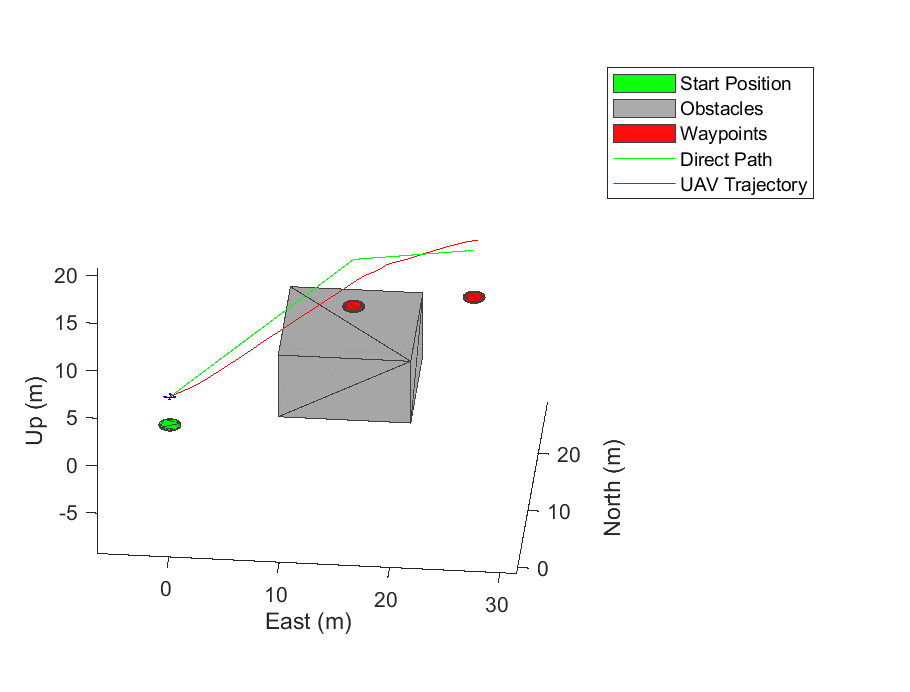
\includegraphics[height=5cm,keepaspectratio]{img/scenario3_fis_paths.eps}
        \caption{Scenario 3 Path taken using ANFIS Drone Control}
        \label{fig:Paths3_fis}
    \end{minipage}
\end{figure}
\begin{figure}[H]
    \centering
    \begin{minipage}[b]{0.45\textwidth}
        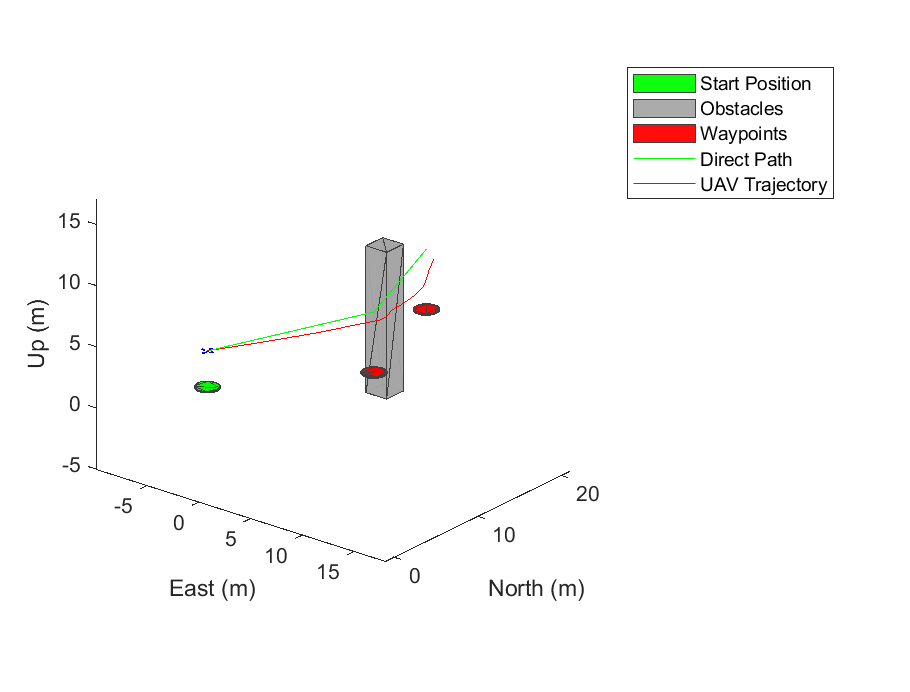
\includegraphics[height=5cm,keepaspectratio]{img/scenario4_pid_paths.eps}
        \caption{Scenario 4 Path taken using PID Drone Control}
        \label{fig:Paths4_pid}
    \end{minipage}
    \hfill
    \begin{minipage}[b]{0.45\textwidth}
        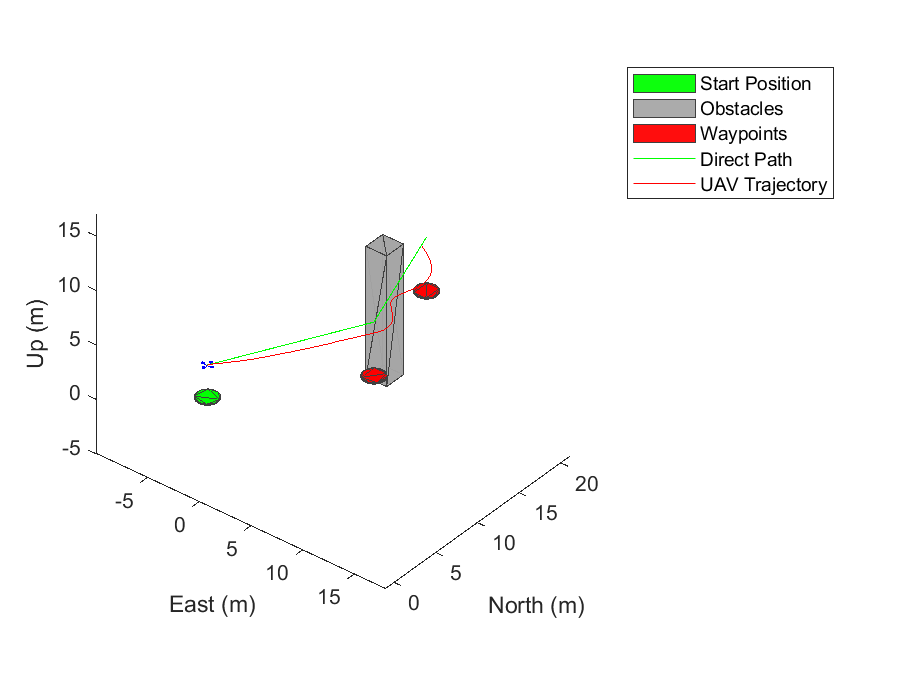
\includegraphics[height=5cm,keepaspectratio]{img/scenario4_fis_paths.eps}
        \caption{Scenario 4 Path taken using ANFIS Drone Control}
        \label{fig:Paths4_fis}
    \end{minipage}
\end{figure}
\begin{figure}[H]
    \centering
    \begin{minipage}[b]{0.45\textwidth}
        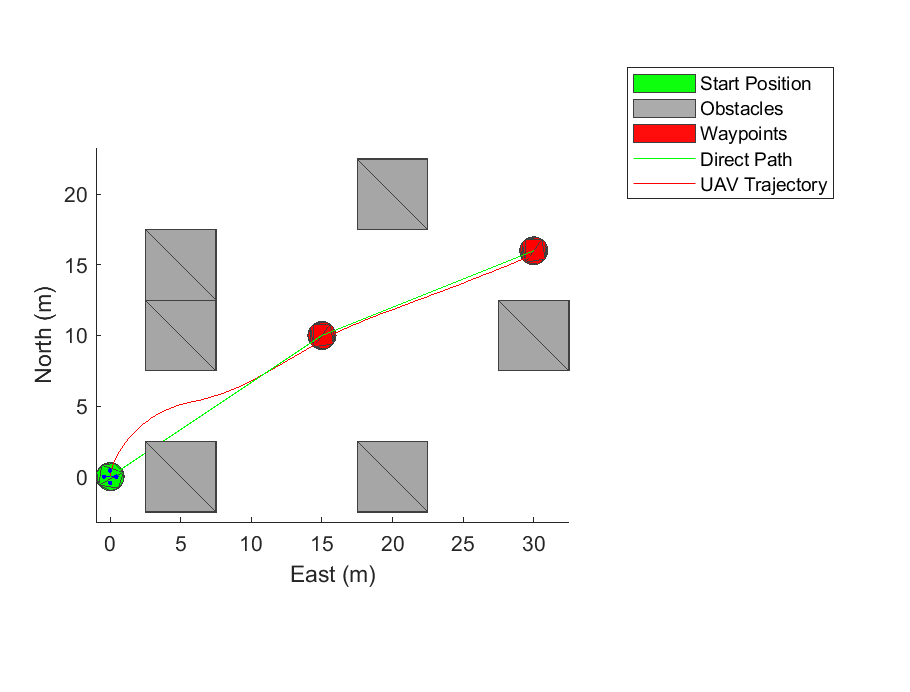
\includegraphics[height=5cm,keepaspectratio]{img/scenario5_pid_paths.eps}
        \caption{Scenario 5 Path taken using PID Drone Control}
        \label{fig:Paths5_pid}
    \end{minipage}
    \hfill
    \begin{minipage}[b]{0.45\textwidth}
        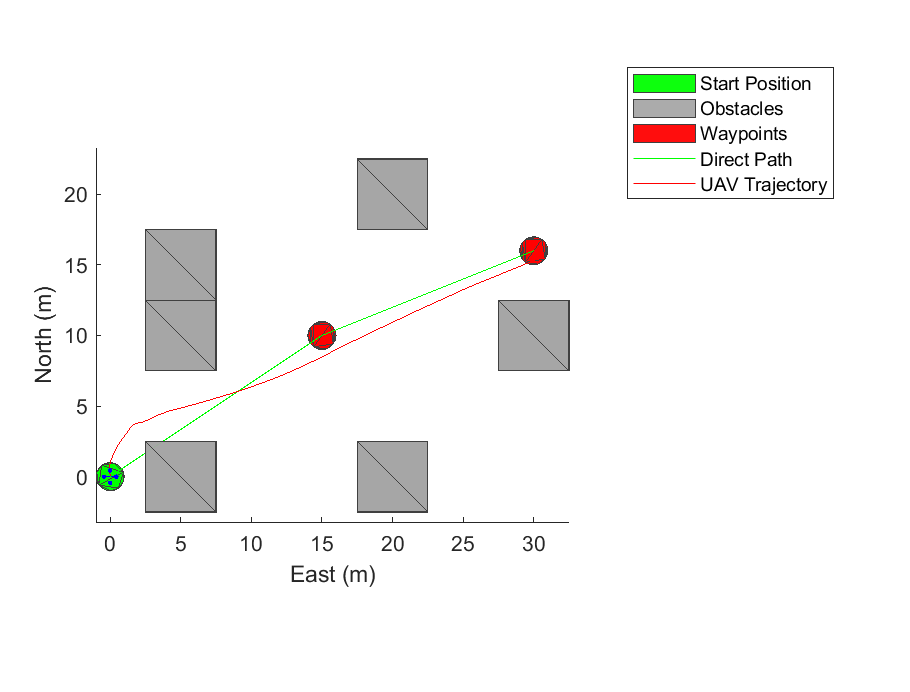
\includegraphics[height=5cm,keepaspectratio]{img/scenario5_fis_paths.eps}
        \caption{Scenario 5 Path taken using ANFIS Drone Control}
        \label{fig:Paths5_fis}
    \end{minipage}
\end{figure}

\end{document}